
In this subsection, we will demonstrate that the diagrams drawn in the last subsections are all related to the amplitudes between boundary states. 

We notice that there is only one apparent length scale in these diagram: in the case of fidelity it is the finite size $L$ for fidelity and $\tau$ for Loschmidt echo. In the absence of the regulators, the conformal invariance can rescale them to $1$ by doing a conformal transformation, thus getting rid of their dependences. Therefore, regulator is necessary in keeping track of the scale dependence in doing the conformal transformation. This is also required by the lattice realization of the systems. 

We work in the folding picture, add small semi-circles to the point where the boundary condition changing operator resides. For the fidelity case, the conformal mapping is depicted in Fig.~\ref{fig:fidel-map} 
\begin{figure}[h]
\centering
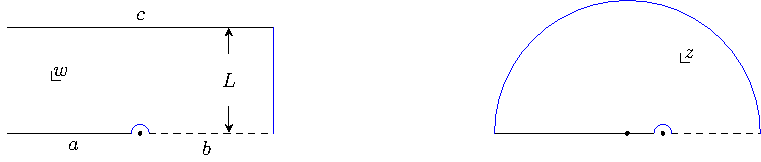
\includegraphics[width=\textwidth]{fig_fidel-map.pdf}
\caption{Mapping from a strip to the upper half plane $w = \frac{L}{\pi} \ln z $. The two black dots represent possible insertion of bcc operators. The dot inside the blue semi-circle is at coordinate $z = 1$, which is the image of point connecting $a$ and $b$ boundaries. The other dot is at $z = 0$, and corresponds to the connection between $a$ and $c$ boundaries at $- \infty$. To evaluate the diagram, we add the outer-semi-circle as the IR cut-off, it can also be regarded as the image of the blue vertical line on the $w$ plane.}
\label{fig:fidel-map}
\end{figure}
If the three boundary conditions $a, b, c$ are all different, then there are two boundary condition changing operators on the real axis. We focus on the one where $a = c$. The two end points of the $\epsilon$ radius semi-circle on the $w$ plane are mapped to
\begin{equation}
\exp( \pm \pi \frac{\epsilon}{ L}  ) \sim 1 \pm \pi \frac{\epsilon}{L} 
\end{equation}
The vertical line at $\text{Re} w = W$ is mapped to $|z| = e^{\pi \frac{W}{L} } \gg 1 $. Since the radius of this larger circle is overwhelming, moving the inner semi-circle on the $z$ plane to the center will not affect the cross ratio to the leading order. The dashed line and solid line are then regarded as two boundary states. The imaginary time evolution is performed in the angular direction and the partition function we are looking for is
\begin{equation}
  Z_{ab} = \langle a | e^{-\pi H } |b \rangle 
\end{equation}

The Loschmidt echo can also be evaluated the same way. We therefore introduce two semi-circles (blue in Fig.~\ref{fig:H-tau_fold}) as regulator and then perform a series conformal transformation as shown in Fig.~\ref{fig:H-tau_fold}. In the $\xi$ plane, we end with the same diagram as fidelity. With one more conformal mapping, it is becomes the cylinder partition function between two boundary states. 

\begin{figure}[htb]
\centering
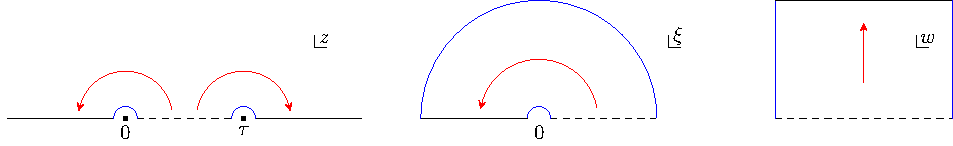
\includegraphics[width=\textwidth]{fig_H-tau_fold}
\caption{Left: diagram of the partition function of Loschimidt echo, where time is the horizontal direction, the dashed(solid) lines are open(gluing) boundary conditions. Red arrows are the directions of Hamiltonian flow that propagates the dashed line boundary state to the solid line boundary state. The blue semi-circles are UV regulators and they are identified as periodic boundaries in the direction perpendicular to the red arrow(equal time slice). Middle: image of the map $\xi = \frac{z}{\tau - z}$. Right: image of $w = \ln \xi$. It is a cylinder by identifying the blue lines and standard radial quantization can be applied. }
\label{fig:H-tau_fold}
\end{figure}

One should however notice that in performing the conformal transformation, we have introduced shifts in free energy. In fact, the free energy in the boundary state calculation gives a positive exponent, meaning a power law increase of the fidelity and echo, which does not make sense. We inspect the shifts in App.~\ref{app:F_correction}, generally speaking it comes from the Schwartzian term and the regulator. 

The amplitude between different boundary states can be computed by the technique presented in App.~\ref{app:lambda_12} and App.~\ref{app:gnd_dn_lambda}, where we set the width of the cylinder to be $\beta$. Adding back the correction in App.~\ref{app:F_correction}, the final result is
\begin{equation}
 - \ln Z_{ab }( \beta ) + \frac{1}{6} \beta 
\end{equation}
where $a,b$ denotes different boundary condition (including the $\lambda$ junction) and $\beta = 2 \ln L$ or  $ 4 \ln \tau$ in the fidelity and echo. 

%%% Local Variables:
%%% TeX-master: "bCFT_paper"
%%% TeX-PDF-mode: t
%%% End:
